\documentclass[14pt]{extarticle}
\usepackage[utf8]{inputenc}
\usepackage[T1]{fontenc}
\usepackage[spanish,es-lcroman]{babel}
\usepackage{amsmath}
\usepackage{amsthm}
\usepackage{physics}
\usepackage{tikz}
\usepackage{float}
\usepackage[autostyle,spanish=mexican]{csquotes}
\usepackage[per-mode=symbol]{siunitx}
\usepackage{gensymb}
\usepackage{multicol}
\usepackage{enumitem}
\usepackage{circuitikz}
\usepackage[left=2.00cm, right=2.00cm, top=2.00cm, 
     bottom=2.00cm]{geometry}
\usepackage{makecell}

\newcommand{\textocolor}[2]{\textbf{\textcolor{#1}{#2}}}
\sisetup{per-mode=symbol}
\DeclareSIUnit[number-unit-product = {\,}]\cal{cal}
\DeclareSIUnit{\dB}{dB}
%\renewcommand{\questionlabel}{\thequestion)}
\decimalpoint
\sisetup{bracket-numbers = false}

\title{\vspace*{-2cm} Actividad - Ejercicios Electricidad \vspace{-5ex}}
\date{}

\begin{document}
\maketitle

\textbf{Indicaciones:} Al inicio de cada hoja que utilices para tu solución, deberás de anotar tu nombre completo.
\par
Resuelve de manera detallada cada uno de los siguientes ejercicios, en donde deberás de indicar el paso (o pasos necesarios) para llegar al resultado.
\par
Cada ejercicio vale un punto si se presenta el desarrollo detallado, hay un ejercicio que vale 2 puntos.
\par
Esta actividad otorgará hasta \textbf{8 puntos}. Si se reporta el resultado directo, sin presentar el desarrollo del ejercicio, éste no aporta puntaje aunque el resultado sea correcto.

\begin{enumerate}
\item Cierto foco tiene una resistencia de \SI{240}{\ohm} cuando se enciende. ¿Cuánta corriente fluirá a través del foco cuando se conecta a \SI{120}{\volt}? que es su voltaje de operación normal.
\item Un calentador eléctrico utiliza \SI{5.0}{\ampere} cuando se conecta a \SI{110}{\volt}. Determina su resistencia.
\item ¿Cuál es el voltaje a través de una parrilla eléctrica que consume \SI{5.0}{\ampere} cuando su resistencia caliente es de \SI{24}{\ohm}?
\item Determina la resistencia equivalente de cuatro resistencias, cuyos valores son: $R_{1} = \SI{3}{\ohm}$, $R_{2} = \SI{1}{\ohm}$, $R_{3} = \SI{4}{\ohm}$ y $R_{4} = \SI{2}{\ohm}$, conectadas primero en  serie y luego en paralelo. Dibuja el diagrama que represente la conexión en cada caso.
\item Siete focos de Navidad con una resistencia de \SI{30}{\ohm} cada uno, se conectan en serie con una diferencia de potencial de \SI{90}{\volt}. Calcula: a) La resistencia equivalente del circuito, b) la intensidad de la corriente que circula por cada resistencia y c) la diferencia de potencial en cada uno de los focos.
\item ¿Qué valor de resistencia se debe conectar en paralelo con una de \SI{20}{\ohm} para hacer una resistencia equivalente de \SI{15}{\ohm}?
\item \textbf{(2 puntos.) }Calcula el valor de voltaje y corriente para cada una de las resistencias del siguiente circuito:
\begin{figure}[H]
    \centering
    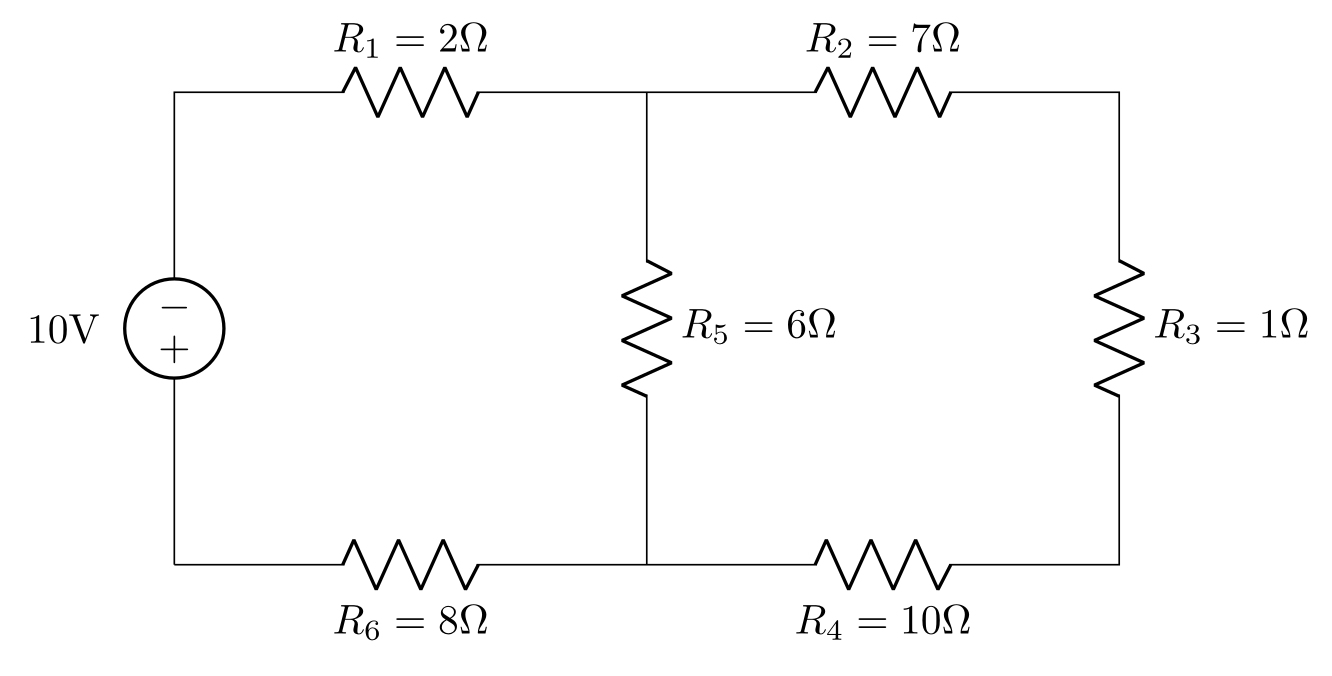
\includegraphics[scale=1.2]{Imagenes/Circuito_01.png}
\end{figure}
Recuerda que tienes que obtener resistencias equivalentes para resolver por partes el circuito, llegando a una sola resistencia $R_{t}$, de donde deberás de extender nuevamente el circuito para calcular la corriente y el voltaje en cada resistencia.
\end{enumerate}

\end{document}